\documentclass{standalone}
    \usepackage{tikz}
    \usepackage{pgfplots}
    \usetikzlibrary{calc}
    \usetikzlibrary{patterns}
    \usetikzlibrary{arrows}
\mathversion{bold}    
% defining the new dimensions and parameters
\newlength{\hatchspread}
\newlength{\hatchthickness}
\newlength{\hatchshift}
\newcommand{\hatchcolor}{}
% declaring the keys in tikz
\tikzset{hatchspread/.code={\setlength{\hatchspread}{#1}},
         hatchthickness/.code={\setlength{\hatchthickness}{#1}},
         hatchshift/.code={\setlength{\hatchshift}{#1}},% must be >= 0
         hatchcolor/.code={\renewcommand{\hatchcolor}{#1}}}
% setting the default values
\tikzset{hatchspread=3pt,
         hatchthickness=0.4pt,
         hatchshift=0pt,% must be >= 0
         hatchcolor=black}
% declaring the pattern
\pgfdeclarepatternformonly[\hatchspread,\hatchthickness,\hatchshift,\hatchcolor]% variables
   {custom north west lines}% name
   {\pgfqpoint{\dimexpr-2\hatchthickness}{\dimexpr-2\hatchthickness}}% lower left corner
   {\pgfqpoint{\dimexpr\hatchspread+2\hatchthickness}{\dimexpr\hatchspread+2\hatchthickness}}% upper right corner
   {\pgfqpoint{\dimexpr\hatchspread}{\dimexpr\hatchspread}}% tile size
   {% shape description
    \pgfsetlinewidth{\hatchthickness}
    \pgfpathmoveto{\pgfqpoint{0pt}{\dimexpr\hatchspread+\hatchshift}}
    \pgfpathlineto{\pgfqpoint{\dimexpr\hatchspread+0.15pt+\hatchshift}{-0.15pt}}
    \ifdim \hatchshift > 0pt
      \pgfpathmoveto{\pgfqpoint{0pt}{\hatchshift}}
      \pgfpathlineto{\pgfqpoint{\dimexpr0.15pt+\hatchshift}{-0.15pt}}
    \fi
    \pgfsetstrokecolor{\hatchcolor}
%    \pgfsetdash{{1pt}{1pt}}{0pt}% dashing cannot work correctly in all situation this way
    \pgfusepath{stroke}
   }

\begin{document}
\huge
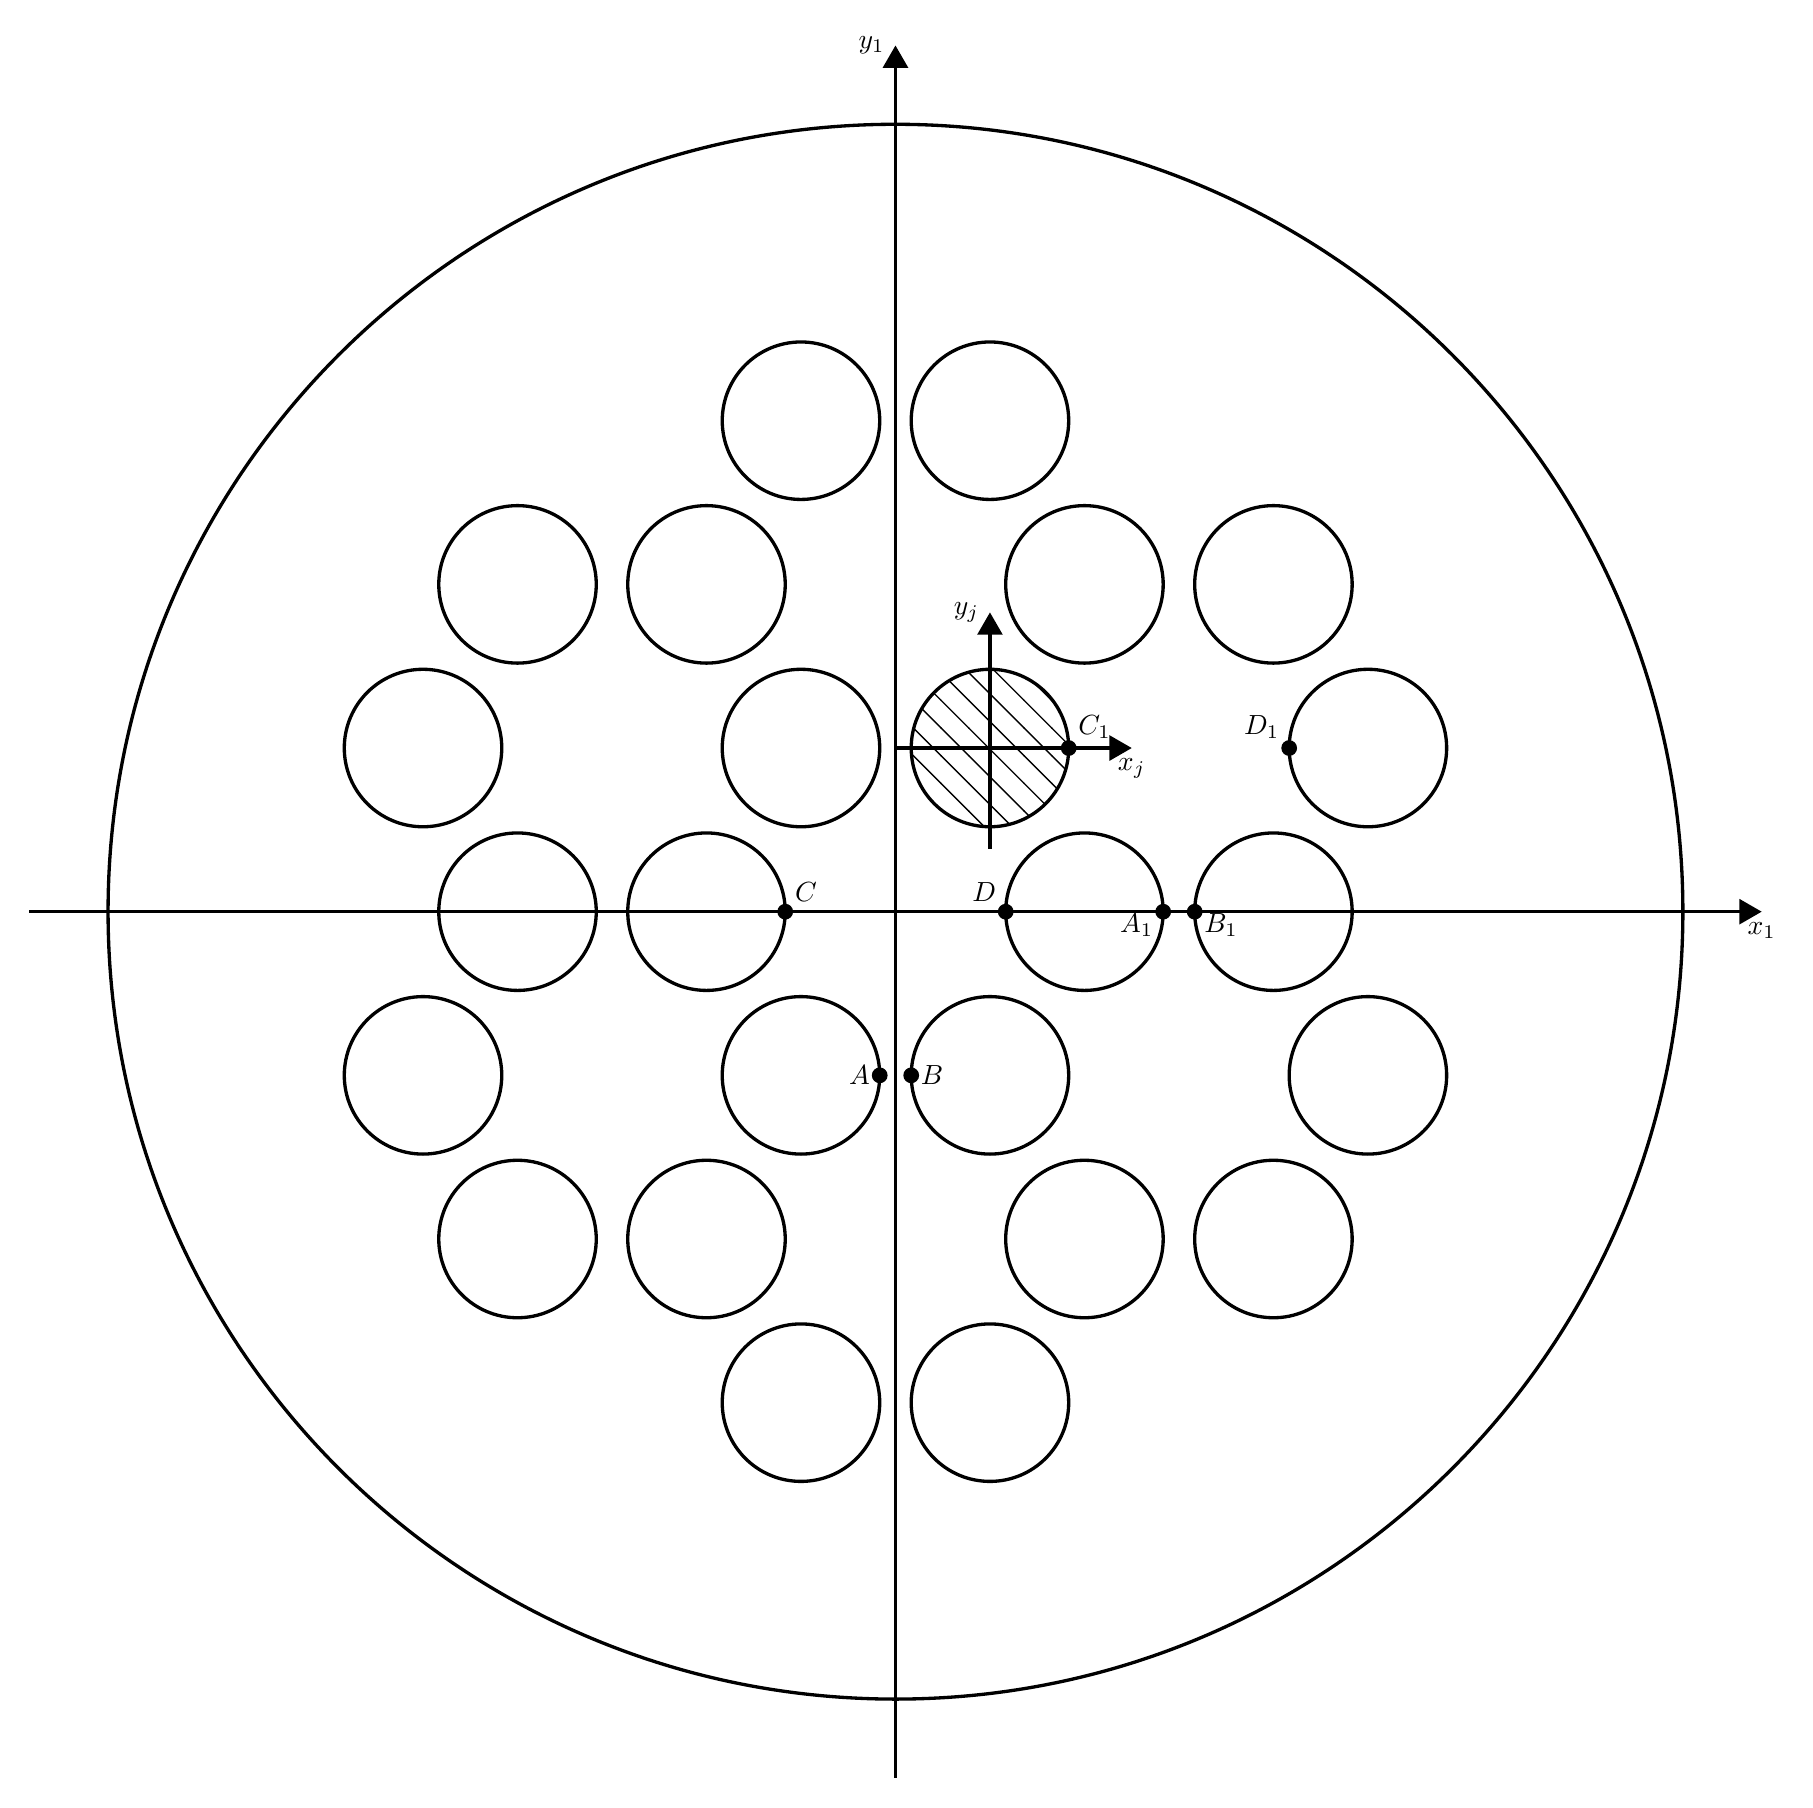
\begin{tikzpicture}[>=triangle 60]
\coordinate (O) at (0,0);
\coordinate (O1) at (2.4, 0);
\coordinate (O2) at (1.2, 2.07846);
\coordinate (O3) at (-1.2, 2.07846);
\coordinate (O4) at (-2.4, 0);
\coordinate (O5) at (-1.2, -2.07846);
\coordinate (O6) at (1.2, -2.07846);
\coordinate (O7) at (6., 2.07846);
\coordinate (O8) at (4.8, 4.15692);
\coordinate (O9) at (2.4, 4.15692);
\coordinate (O10) at (4.8, 0.);
\coordinate (O11) at (1.2, 6.23538);
\coordinate (O12) at (-1.2, 6.23538);
\coordinate (O13) at (-2.4, 4.15692);
\coordinate (O14) at (-4.8, 4.15692);
\coordinate (O15) at (-6., 2.07846);
\coordinate (O16) at (-4.8, 0.);
\coordinate (O17) at (-6., -2.07846);
\coordinate (O18) at (-4.8, -4.15692);
\coordinate (O19) at (-2.4, -4.15692);
\coordinate (O20) at (2.4, -4.15692);
\coordinate (O21) at (-1.2, -6.23538);
\coordinate (O22) at (1.2, -6.23538);
\coordinate (O23) at (6., -2.07846);
\coordinate (O24) at (4.8, -4.15692);

\coordinate (A) at (-0.2, -2.07846);
\coordinate (B) at (0.2, -2.07846);
\coordinate (C) at  (-1.4, 0);
\coordinate (D) at (1.4, 0);
\coordinate (A1) at (3.4, 0);
\coordinate (B1) at (3.8, 0);
\coordinate (C1) at (2.2, 2.07846);
\coordinate (D1) at (5.0, 2.07846);

\draw[very thick] (O) circle (10.0);
\draw[->,very thick] (-11,0) -- (11,0) node[below] {$x_1$};
\draw[->,very thick] (0,-11) -- (0,11) node[left] {$y_1$};

\draw[->,very thick] (0,2.07846) -- (3.0,2.07846) node[below] {$x_j$};
\draw[->,very thick] (1.2,0.8) -- (1.2,3.8) node[left] {$y_j$};

\draw[very thick] (O1) circle (1.0);
\draw[very thick] (O2) circle (1.0);
\draw[very thick] (O3) circle (1.0);
\draw[very thick] (O4) circle (1.0);
\draw[very thick] (O5) circle (1.0);
\draw[very thick] (O6) circle (1.0);
\draw[very thick] (O7) circle (1.0);
\draw[very thick] (O8) circle (1.0);
\draw[very thick] (O9) circle (1.0);
\draw[very thick] (O10) circle (1.0);
\draw[very thick] (O11) circle (1.0);
\draw[very thick] (O12) circle (1.0);
\draw[very thick] (O13) circle (1.0);
\draw[very thick] (O14) circle (1.0);
\draw[very thick] (O15) circle (1.0);
\draw[very thick] (O16) circle (1.0);
\draw[very thick] (O17) circle (1.0);
\draw[very thick] (O18) circle (1.0);
\draw[very thick] (O19) circle (1.0);
\draw[very thick] (O20) circle (1.0);
\draw[very thick] (O21) circle (1.0);
\draw[very thick] (O22) circle (1.0);
\draw[very thick] (O23) circle (1.0);
\draw[very thick] (O24) circle (1.0);

\fill (A) circle (0.1);
\fill (B) circle (0.1);
\fill (C) circle (0.1);
\fill (D) circle (0.1);
\fill (A1) circle (0.1);
\fill (B1) circle (0.1);
\fill (C1) circle (0.1);
\fill (D1) circle (0.1);

\fill[pattern=custom north west lines,hatchspread=10pt,hatchthickness=0.5pt,hatchcolor=black] (O2) circle(1.0);

\node[left] at (A) {$A$};
\node[right] at (B) {$B$};
\node[above right] at (C) {$C$};
\node[above left] at (D) {$D$};
\node[below left] at (3.4,0.1) {$A_1$};
\node[below right] at (3.8,0.1) {$B_1$};
\node[above right] at (C1) {$C_1$};
\node[above left] at (D1) {$D_1$};

\end{tikzpicture}
\end{document}

%%% Local Variables: 
%%% mode: latex
%%% TeX-master: t
%%% End: 
